% !TEX TS-program = pdflatex
% !TEX encoding = UTF-8 Unicode

% This file is a template using the "beamer" package to create slides for a talk or presentation
% - Talk at a conference/colloquium.
% - Talk length is about 20min.
% - Style is ornate.

% MODIFIED by Jonathan Kew, 2008-07-06
% The header comments and encoding in this file were modified for inclusion with TeXworks.
% The content is otherwise unchanged from the original distributed with the beamer package.

\documentclass{beamer}
\usepackage{tikz}
\usepackage{tikz-cd}


\mode<presentation>
{
  \usetheme{Warsaw}

  \setbeamercovered{transparent}
  % or whatever (possibly just delete it)
}


\usepackage[english]{babel}
\usepackage[utf8]{inputenc}
\usepackage{times}
\usepackage[T1]{fontenc}

\title[Short Paper Title] % (optional, use only with long paper titles)
{La méthode des moindres carrés, la gaussienne et le concept d'efficience de marché}
\author[Author, Another] % (optional, use only with lots of authors)
{Clément Dell'Aiera}
% - Give the names in the same order as the appear in the paper.
% - Use the \inst{?} command only if the authors have different
%   affiliation.

\institute[Universities of Somewhere and Elsewhere] 
{ ENS Rennes
  }

\date[CFP 2003] % (optional, should be abbreviation of conference name)
{Journée 4A, 2014}

\AtBeginSubsection[]
{
  \begin{frame}<beamer>{Outline}
    \tableofcontents[currentsection,currentsubsection]
  \end{frame}
}


% If you wish to uncover everything in a step-wise fashion, uncomment
% the following command: 

%\beamerdefaultoverlayspecification{<+->}


\begin{document}

\begin{frame}
  \titlepage
\end{frame}

\begin{frame}{}
  \tableofcontents
  % You might wish to add the option [pausesections]
\end{frame}


% Structuring a talk is a difficult task and the following structure
% may not be suitable. Here are some rules that apply for this
% solution: 

% - Exactly two or three sections (other than the summary).
% - At *most* three subsections per section.
% - Talk about 30s to 2min per frame. So there should be between about
%   15 and 30 frames, all told.

% - A conference audience is likely to know very little of what you
%   are going to talk about. So *simplify*!
% - In a 20min talk, getting the main ideas across is hard
%   enough. Leave out details, even if it means being less precise than
%   you think necessary.
% - If you omit details that are vital to the proof/implementation,
%   just say so once. Everybody will be happy with that.

\section{De la méthode du milieu à la loi normale}

\begin{frame}
\begin{figure}[!h]\centering
\includegraphics[scale=0.175]{Gauss2.jpg}
\caption{Gauss}
\label{fig:Gauss2}
\end{figure}
\end{frame}

\begin{frame}
\begin{figure}[!h]\centering
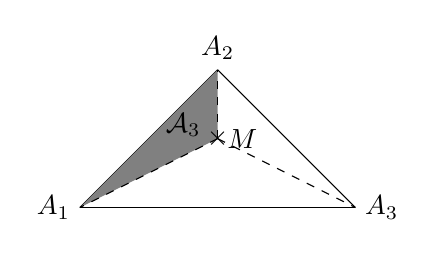
\begin{tikzpicture}[scale = 1.75]
\draw (0,0) -- (1,1);
\draw (0,0) -- (2,0);
\draw (1,1) -- (2,0);
\fill[gray] (0,0) -- (1,1) -- (1,0.5) -- cycle;
\draw[dashed] (1,0.5) -- (2,0);
\draw[dashed] (1,0.5) -- (0,0);
\draw[dashed] (1,0.5) -- (1,1);
\draw (0.75,0.6) node{$\mathcal A_3$};
\draw (0,0) node[left]{$A_1$} ;
\draw (2,0)  node[right]{$A_3$};
\draw (1,1)  node[above]{$A_2$};
\draw (1,0.5) node{$\times$};
\draw (1,0.5) node[right]{$M$};
\end{tikzpicture}
\caption{\textbf{Point de Lemoine.} L'aire grisée est proportionnelle à la coordonnée barycentrique de $M$ relative à $A_3$.}
\label{Lemoine}
\end{figure}
\end{frame}

\begin{frame}
\begin{figure}[!h]\centering

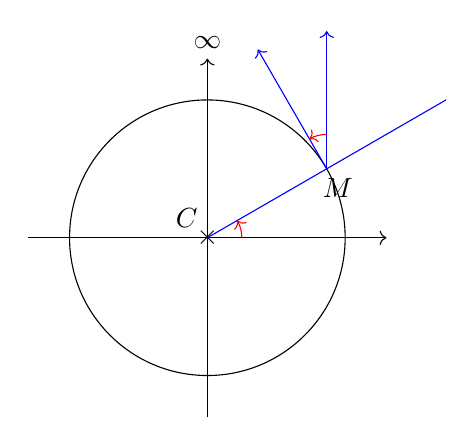
\begin{tikzpicture}[scale = 1.75]
\draw (0,0) circle (1);
\draw (0,0) node{$\times$};
\draw (0,0) node[above left]{$C$};
\draw[->] (0,-1.3) -- (0,1.3);
\draw[->] (-1.3,0) -- (1.3,0);
\draw (0,1.3) node[above]{$\infty$};
\draw[red,->] (0.25,0) arc (0:30:0.25);

\draw[blue] (0,0) -- ++ (2*0.866,2*0.5) ;
\draw (1.3*0.866,0.5) node[below left]{$M$};
\pause
\draw[blue,->] (0.866,0.5) -- ++ (-0.5,0.866);
\draw[blue,->] (0.866,0.5) -- ++ (0,1);
\pause

\draw[red,->] (0.866,0.5+0.25) arc (90:120:0.25);

\end{tikzpicture}
\caption{\textbf{Latitude.} La latitude peut se mesurer en visant l'angle que fait l'étoile polaire avec l'horizon. }
\label{Latitude}
\end{figure}
\end{frame}

\begin{frame}
\begin{figure}[!h]\centering
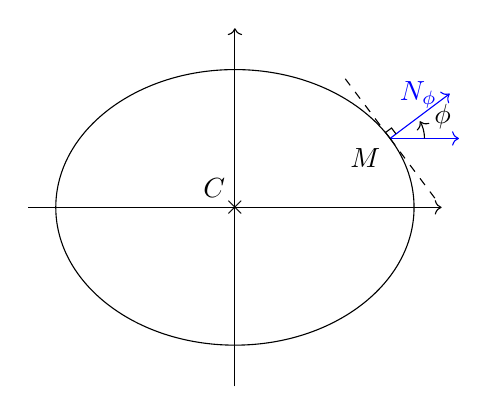
\begin{tikzpicture}[scale = 1.75]
\draw (0,0) ellipse (1.3 and 1);
\draw (0,0) node{$\times$};
\draw (0,0) node[above left]{$C$};
\draw[->] (0,-1.3) -- (0,1.3);
\draw[->] (-1.5,0) -- (1.5,0);

\draw (1.3*0.866,0.5) node[below left]{$M$};

\draw[blue,->] (1.3*0.866,0.5) -- ++ (0.5*0.866,0.5*1.3*0.5);
\draw[blue] (1.3*0.866,1.3*0.5) node[above right]{$N_\phi$};
\draw[blue,->] (1.3*0.866,0.5) -- ++ (0.5,0);
\draw[->] (1.3*0.866+0.25,0.5) arc (0:30:0.25);
\draw (1.3*0.866+0.25,0.5) node[above right]{$\phi$};

\draw[dashed] (1.3*0.866,0.5)-- ++ (0.5*1.3*0.5,-0.5*0.866);
\draw[dashed] (1.3*0.866,0.5)-- ++ (-0.5*1.3*0.5,0.5*0.866);
\draw (1.3*0.866-0.05*1.3*0.5,0.5+0.05*0.866) -- ++ (0.05*0.866,0.05*1.3*0.5) -- ++ (0.05*1.3*0.5,-0.05*0.866) ;
\end{tikzpicture}
\caption{\textbf{Forme de la Terre.} La latitude $\phi$ est donnée par l'angle entre la normale avec le plan de l'ecliptique. }
\label{Ellipse}
\end{figure}
\end{frame}

\section{Lois des erreurs et lois stables}
\begin{frame}
\begin{figure}[!h]\centering
\includegraphics[scale=0.25]{Laplace.png}
\caption{Loi de l'erreur de Laplace en faisant varier le paramètre $m$ : plus il est élevé, plus l'erreur se disperse}
\label{fig:Laplace}
\end{figure}
\end{frame}

\begin{frame}
\begin{figure}[!h]\centering
\includegraphics[scale=0.25]{Gaussienne.png}
\caption{Loi de l'erreur gaussienne en faisant varier le paramètre $h$ : plus il est élevé, plus l'erreur se disperse}
\label{fig:Gaussienne}
\end{figure}
\end{frame}

\begin{frame}
\begin{figure}[!h]\centering
\includegraphics[scale=0.25]{Stables.jpeg}
\caption{Densité de lois stables. Plus la courbe est bleue, plus $\alpha$ se rapproche de $2$, et l'on retrouve la loi de Gauss.}
\label{fig:Stables}
\end{figure}
\end{frame}




\end{document}


